\documentclass{standalone}
\usepackage{tikz}
\usepackage{pgfplots}
\pgfplotsset{compat=1.16}

\begin{document}
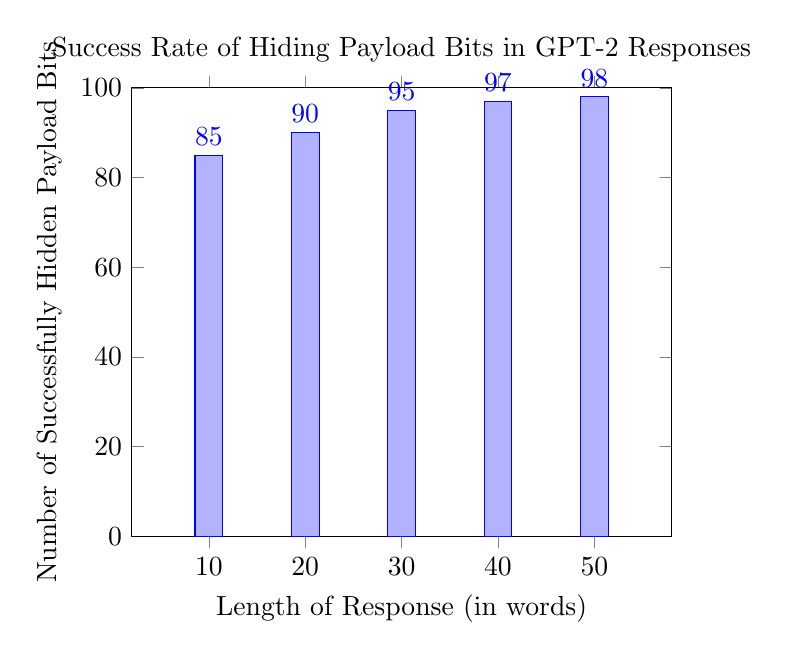
\begin{tikzpicture}
    \begin{axis}[
        ybar,
        symbolic x coords={10, 20, 30, 40, 50},
        xtick=data,
        nodes near coords,
        nodes near coords align={vertical},
        ylabel={Number of Successfully Hidden Payload Bits},
        xlabel={Length of Response (in words)},
        title={Success Rate of Hiding Payload Bits in GPT-2 Responses},
        enlarge x limits=0.2,
        ymin=0,
        ymax=100
    ]
        \addplot coordinates {(10, 85) (20, 90) (30, 95) (40, 97) (50, 98)};
    \end{axis}
\end{tikzpicture}
\end{document}